\chapter{Práctica: Vacuum}\label{cap.roomba}
En este capítulo se expondrá el desarrollo de una nueva práctica para la plataforma de JdeRobot, que se llamará ``Vacuum''. En este capítulo se aborda el desarrollo de la infraestructura, aplicación gráfica, una gráfica de la derivada del porcentaje, así como el árbitro creado y la solución llevada a cabo.\\

\section{Enunciado de la práctica}
El objetivo de esta práctica (llamada vacuum) es que una aspiradora robótica sea capaz de limpiar de forma autónoma la mayor cantidad de superficie posible en una casa. La aspiradora no tendrá ninguna forma de obtener su posición en el mundo, ya que el propósito de la práctica es que el algoritmo que se lleve a cabo sea sin autolocalización. El único dato que conocerá la aspiradora es su orientación.  Además, esta aspiradora posee un sensor láser, que le permite medir la distancia a la que se sitúan los obstáculos. Esta aspiradora tiene un actuador de movimiento que se basa en velocidad lineal y velocidad de giro. Todos estos elementos nos deberán permitir realizar un algoritmo de pilotaje para recorrer la casa.\\

En esta práctica el alumno deberá programar el algoritmo capaz de limpiar un gran porcentaje de la casa sin autolocalización. En la interfaz gráfica se puede visualizar un mapa de la casa, así como la posición de la aspiradora en el mapa y los lugares por donde ha pasado. Este mapa no estará disponible para realizar la solución sin autolocalización, el mapa únicamente se utiliza para facilitar el trabajo al alumno. \\

El algoritmo responde a un control reactivo, que en cada instante actuará en función de los datos de los sensores o del algoritmo que se planifique en cada instante. El control reactivo permitirá controlar en todo momento el entorno que rodea al robot y responder ante situaciones imprevistas.\\

\section{Diseño general de la práctica}
En esta sección se describirá el diseño general que tiene la práctica, es decir, en qué partes se divide el comportamiento de la misma haciendo que sea más sencilla su creación, ya que se divide en tareas más simples.\\

\subsection{Diseño general}
Como ya vimos en la práctica anterior, las prácticas de JdeRobot se llevan a cabo sobre el entorno de prácticas JdeRobot/Academy. Gracias a este entorno el alumno puede centrarse únicamente en el desarrollo del algoritmo que da solución al caso que se plantea en cada práctica. Al igual que en la anterior práctica, se explicará cómo se ha creado el entorno de esta práctica por encima, y se profundizará en esto en los puntos siguientes. \\

El primer paso que se ha tenido en cuenta es la creación de la infraestructura de la práctica, lo que abarca la creación de los modelos o modificación de los ya existentes, así como de los plugins de los que hacen uso los modelos. Además, se creará el mundo por donde navegará nuestro robot. Este mundo estará formado por los modelos que se han creado o de los que se haga uso. Como explicamos en la práctica anterior, se creará el archivo de configuración (con extensión .cfg), que permite a nuestra aplicación comunicarse con gazeboserver.\\

Además, se creará la interfaz gráfica, que servirá como visor, ayudando al alumno en la resolución de las prácticas. En este visor podremos ver un mapa de la casa en la que se sitúa el robot y la posición del mismo dentro de la casa.\\

En tercer lugar, se creará un árbitro para la evaluación de la práctica. Este árbitro posee un visor gráfico como en la GUI. En este visor se mostrarán diferentes parámetros que sirven para la evaluación de la práctica.\\

Por último, se ha llevado a cabo la creación de una gráfica que muestra la derivada del porcentaje que recorre el robot en función del tiempo. Esta gráfica mostrará cada cierto periodo de tiempo esta derivada, lo que permite ver la evolución del algoritmo en el tiempo.\\

Además, el alumno dispondrá de un archivo (MyAlgorithm.py), que servirá como plantilla para que el alumno programe la solución de navegación del robot. En la descripción de esta práctica se incluye una breve explicación del algoritmo que se ha programado como solución.\\

En los próximos apartados se profundizará en todos estos puntos que hemos mencionado. Se describirán en mayor profundidad en los apartados 5.3 (infraestructura), 5.4 (interfaz gráfica), 5.5 (gráfica de la derivada del porcentaje), 5.6 (árbitro), y 5.7 (solución).\\

\subsection{Hilos de ejecución de la práctica}
La práctica emplea hilos de ejecución para poder realizar diferentes tareas al mismo tiempo, ya que como habíamos mencionado antes se divide el comportamiento en tareas más sencillas. Esta práctica emplea varios procesos:

\begin{itemize}
\item Hilo de control: Es el encargado de actualizar los datos de los sensores y los actuadores a través de las interfaces ICE. El tiempo de refresco de este hilo es crucial, y tiene que ser un periodo de tiempo muy corto, ya que este componente se encarga de establecer la velocidad y la dirección del robot en todo momento, así como de actualizar los datos de los sensores que son muy importantes para la solución de la práctica. Si este tiempo fuera muy grande, las decisiones que modifican la navegación del robot podrían ser incorrectas. En el caso de esta práctica el hilo de control de actuadores y sensores se actualizará cada vez que se actualiza la GUI, es decir, cada 50 ms.
\item Hilo de la interfaz gráfica de usuario (GUI): Este hilo es el encargado de actualizar la interfaz gráfica. También consta de los manejadores de eventos del GUI, que son los encargados de ejecutar el código del fichero MyAlgorithm.py. El intervalo de actualización de la interfaz debe ser pequeño, ya que se tiene que mostrar la posición del robot en el mapa que se muestra en la interfaz en tiempo real. Este intervalo de tiempo es de 50 ms.
\item Hilo del árbitro: Este hilo actualiza los parámetros que se muestran en el árbitro. El intervalo de actualización de este hilo debe ser pequeño, ya que como en el caso de la GUI, tendremos que garantizar al usuario que los parámetros que le mostramos son actuales. Este hilo de ejecución se actualiza cada 50 ms.
\item Hilo de la gráfica de la derivada del porcentaje: Este hilo se encarga de actualizar la gráfica de la derivada del porcentaje en función del tiempo. Es necesario que esta gráfica se actualice en un periodo corto de tiempo, puesto que da información del porcentaje en el tiempo. Por ello, este hilo se actualiza cada 50 ms.
\end{itemize}

\subsection{Cómo ejecutar la práctica}
La práctica ``vacuum'' se puede ejecutar de dos formas diferentes como sucedía en la anterior práctica, con script o sin script. El script se ha creado para facilitar al alumno la ejecución de la práctica, pero no es necesario usarlo.\\

Si no se quiere emplear el script se pueden abrir cuatro terminales y escribir lo siguiente en cada uno de ellos para ejecutar la práctica:

\begin{itemize}
\item Lanzar Gazebo: gazebo Vacuum.world
\item Ejecutar la práctica y lanzar la interfaz gráfica (GUI): python2 vacuum.py --Ice.Config=vacuum.cfg
\item Lanzar la gráfica de la derivada del porcentaje: python2 graphicPercentaje.py --Ice.Config=vacuum.cfg
\item Lanzar el árbitro: python2 referee.py --Ice.Config=vacuum.cfg
\end{itemize}

Si queremos emplear el script (run\_it.sh) para poder ejecutar la práctica podemos ejecutar la práctica sin lanzar Gazebo por defecto o lanzándolo. Si se va a emplear una máquina con pocas capacidades, es mejor no lanzar Gazebo, ya que consume muchos recursos. La práctica se puede ejecutar de la siguiente forma:\\

\begin{itemize}
\item Ejecución sin ver el mundo de Gazebo: ./run\_it.sh
\item Ejecución viendo el mundo de Gazebo: ./run\_it.sh GUI
\end{itemize}

\section{Infraestructura}
En este apartado se describirá el entorno creado para realizar la práctica “vacuum”. Además, se describirá el robot que se ha utilizado en esta práctica, así como el entorno por el que se mueve este robot. También se explicarán los sensores y actuadores que tiene el robot.\\

\subsection{Roomba}
El robot que se ha empleado en esta práctica es el robot Roomba de la serie 500, que fue comercializado por la empresa iRobot (en Estados Unidos). Esta aspiradora robótica está equipada con un conjunto de sensores con los que explorar sus alrededores y unos actuadores que le permiten moverse adecuadamente por su entorno. Los modelos de Roomba de esta serie poseen sensores infrarrojos, un sensor detector de suciedad, un sensor detector de desniveles, y cuentan además con un bumper. \\

En el caso de la práctica, se empleó el modelo de Roomba de JdeRobot, que no tiene detector de desniveles debido a que el escenario de nuestra práctica no contiene desniveles; y tampoco tiene detector de suciedad, puesto que no se ha simulado la suciedad en el mundo de Gazebo ya que el objetivo era realizar el algoritmo de navegación. En nuestro modelo de Roomba tenemos un sensor bumper, que nos permite detectar los choques con objetos; y un sensor láser, que nos permite medir la distancia a los objetos. Este sensor láser es capaz de hacer un barrido de 180 grados, con precisión de 1 grado. Además, este robot posee sensores de odometría, los cuales le permiten conocer la posición en la que se encuentra el robot en cada momento.\\

El robot Roomba de la serie 500 posee una anchura de 340 milímetros, 92 milímetros de altura, y un peso de 3.6 kg. El modelo Roomba de JdeRobot mide aproximadamente 330 mm de ancho, 90 mm de altura, y un peso de 2.5 kg.\\

\begin{figure}[H]
  \begin{center}
    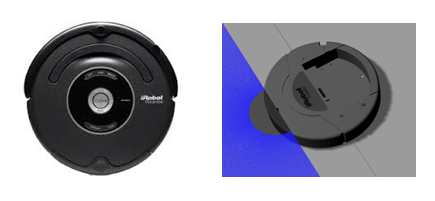
\includegraphics[width=0.6\textwidth]{figures/Vacuum/Roombas.png}
		\caption{Roomba de iRobot y modelo Roomba en Gazebo}
		\label{fig.roombas}
		\end{center}
\end{figure}

\subsection{Sensor láser}
En la parte frontal del robot se ha instalado un sensor láser. Este sensor se utilizará ampliamente en el algoritmo de la práctica. Este sensor láser está compuesto por un array de 180 láseres, esto supone que vamos a tener un láser que puede medir distancia alrededor de 180 grados. Esta cualidad nos permite detectar obstáculos en estos 180 grados, y poder determinar dónde se encuentra aproximadamente. Las medidas de distancia que nos devuelve el láser están en milímetros.\\

Una vez más la plataforma JdeRobot encapsula la complejidad de este sensor y nos devuelve los datos que ofrece el mismo, es decir, los datos de distancia de cada posición del array del láser. \\

\subsection{Sensor bumper}
El sensor bumper es un sensor de contacto que nos permite detectar una colisión con un objeto. Esto va a ser muy útil para realizar el algoritmo de esta práctica. Este sensor lo que hace es comprobar el número de contactos con el entorno y si dicho número es mayor que cero es porque el robot ha chocado con algún objeto. La plataforma JdeRobot nos abstrae de realizar el comportamiento complejo de este sensor, y nos permite conocer si ha habido algún choque con algún obstáculo de manera sencilla. La forma que tiene JdeRobot de comunicarnos si hay un choque o no es devolviéndonos un 0 o un 1 en función de si existe choque o no. Si el robot se ha chocado con algún objeto, entonces el bumper nos devolverá un 1. Por el contrario, si el robot no colisiona con ningún obstáculo, entonces el bumper nos dará como resultado un 0.\\

\subsection{Plugins}
Como mencionamos en la práctica anterior, JdeRobot consta de un amplio repertorio de drivers que facilitan la comunicación con los sensores y actuadores. En esta práctica, en concreto, se han utilizado cuatro drivers: 

\begin{itemize}
\item pose3di: Los componentes harán uso de este plugin para obtener su posición en tiempo real. Además, este plugin se emplea para modificar la posición de los componentes.
\item motorsi: Este plugin interactúa con el componente, dotándole de velocidad, tanto velocidad de tracción como velocidad de rotación y modifica los datos de la interfaz de usuario.
\item Laseri: Este plugin será usado por los componentes para poder obtener información de la distancia que hay hasta los obstáculos.
\item Bumperi: El componente podrá usar este plugin para recolectar información acerca de su situación de colisión con otro objeto cualquiera.
\end{itemize}

\subsection{Modelo House}
El propósito de esta práctica es que el robot Roomba sea capaz de recorrer la superficie del suelo de una casa. Por lo tanto, será necesario crear un modelo de casa para poder interactuar en ella. Hemos empleado el modelo de casa que empleo Juan Navarro [18] en su proyecto en el mundo GrannyAnnie.world (se puede observar en la siguiente imagen), pero hemos realizado algunas modificaciones. \\

\begin{figure}[H]
  \begin{center}
    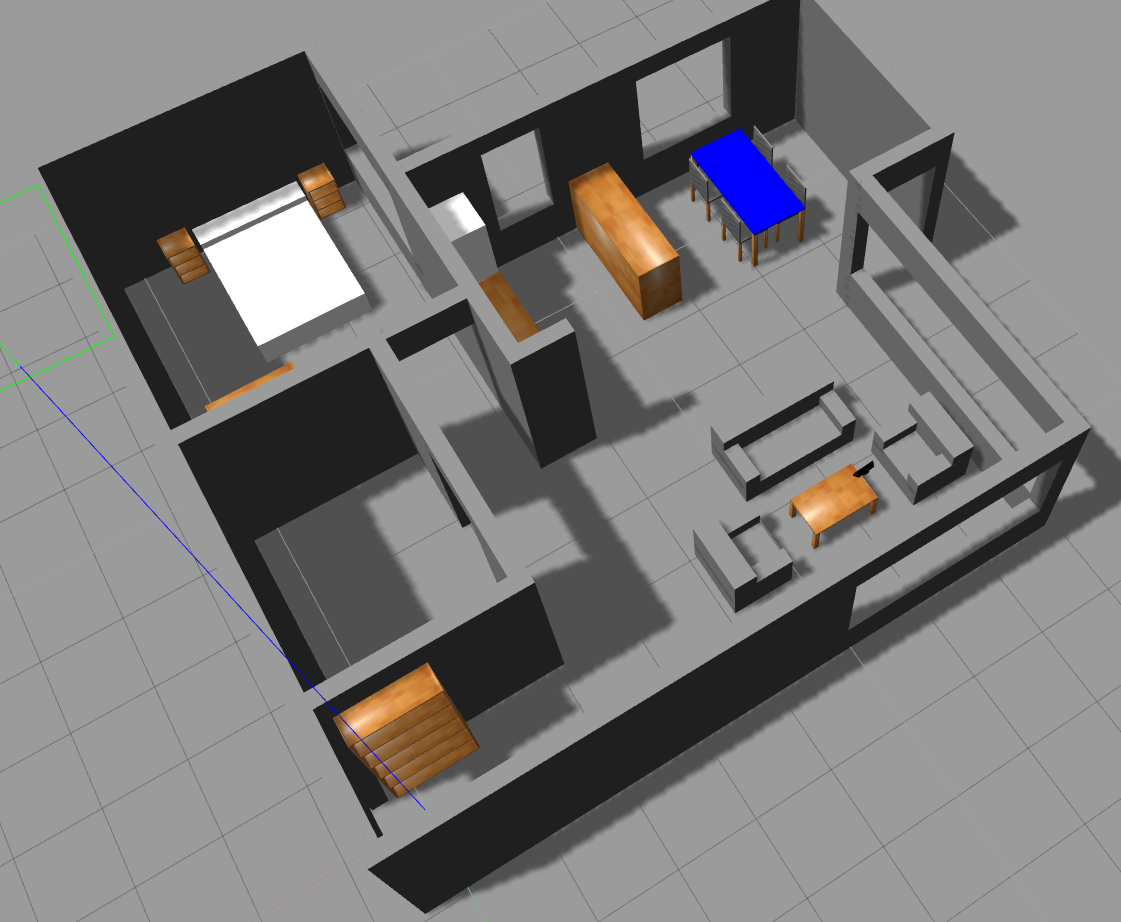
\includegraphics[width=0.6\textwidth]{figures/Vacuum/ModeloCasa_antiguo.png}
		\caption{Mundo GrannyAnnie.world en Gazebo}
		\label{fig.modelocasa_antiguo}
		\end{center}
\end{figure}

Este modelo se ha tenido que modificar puesto que había puertas que daban al exterior de la casa, entonces si pusiéramos a nuestra aspiradora a recorrer la casa se podría salir de la misma y no queremos que suceda esto. Además, se modificó el modelo de la casa debido a que había alguna pared que tenía mal la malla de colisiones, esto hacía que el robot pudiera atravesar algunas paredes. Este era un problema puesto que la casa tiene que ser lo más realista posible, por lo que se modificó la malla de colisiones en algunas zonas de la casa. Además, se modificaron las masas del inmobiliario incrementando su valor. Esto se debe a que la masa que tenían anteriormente no era suficiente y la aspiradora al colisionar con los muebles (mesas, sillones, etc) los desplazaba. El nuevo modelo de casa se llama “house\_int2” y lo podemos ver a continuación.\\

\begin{figure}[H]
  \begin{center}
    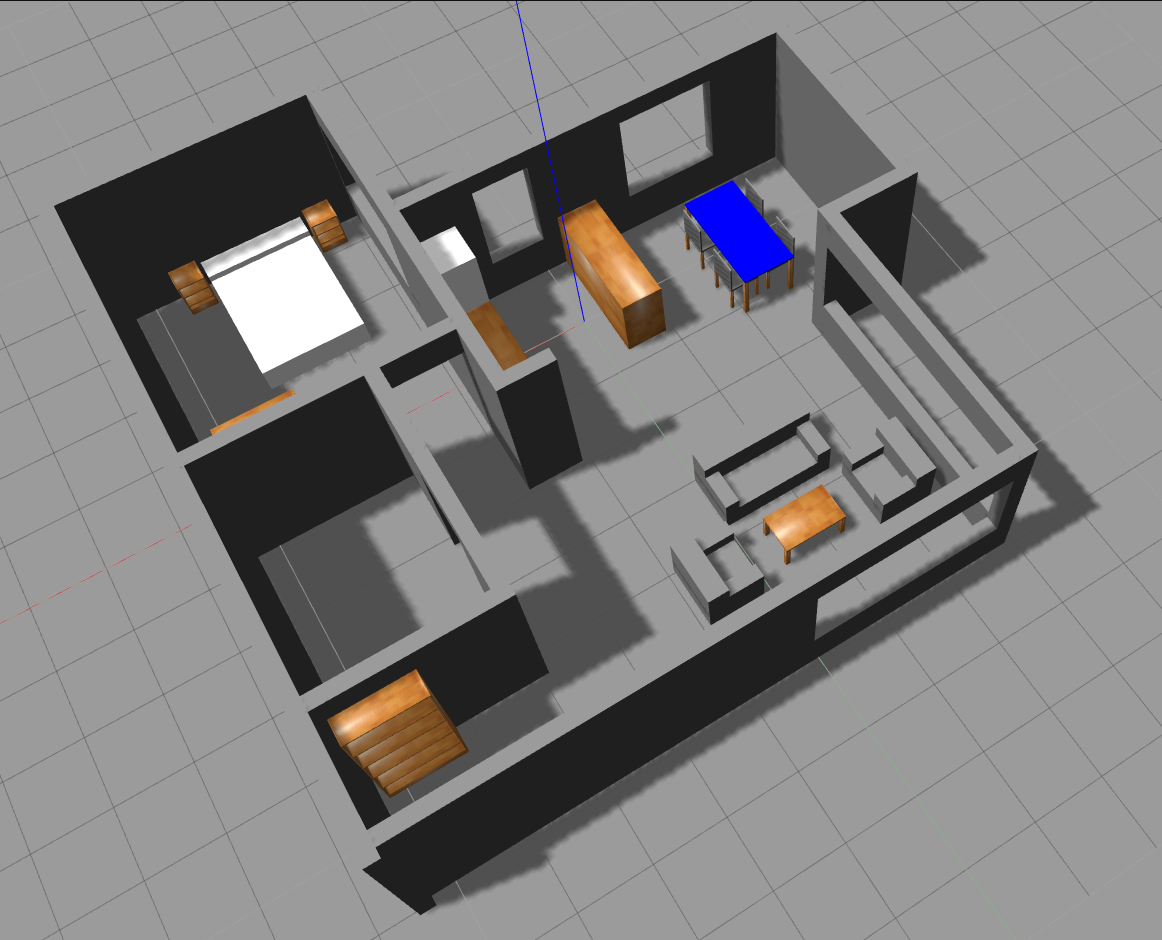
\includegraphics[width=0.6\textwidth]{figures/Vacuum/casa.png}
		\caption{Modelo house\_int2 en Gazebo}
		\label{fig.casa}
		\end{center}
\end{figure}

\subsection{Mundo de Gazebo}
Si queremos ver el comportamiento de la aspiradora dentro de la casa, antes debemos crear un mundo de Gazebo que esté formado por el modelo de la casa ``house\_int2'' y el modelo de aspiradora ``Roomba''. Por este motivo se ha creado un mundo llamado ``Vacuum.world''. Este archivo tiene el siguiente aspecto:

\vspace{20pt}
	\begin{lstlisting}[frame=single]
<?xml version="1.0" ?>
  <sdf version='1.4'>
    <world name=' Vacuum '>
    <include>
      <uri>model://roomba</uri>
        <pose>-1 1.5 0 0 0 0</pose>
    </include>
    <include>
      <uri>model://house_int2</uri>
        <pose>0 0 0 0 0 0</pose>
    </include>
    <include>
      <uri>model://ground_plane</uri>
   </include>

   <light name='sun' type='directional'>
       <cast_shadows>1</cast_shadows>
       <pose>0 0 10 0 -0 0</pose>
       <diffuse>0.8 0.8 0.8 1</diffuse>
       <specular>0.2 0.2 0.2 1</specular>
       <attenuation>
       <range>1000</range>
       <constant>0.9</constant>
       <linear>0.01</linear>
       <quadratic>0.001</quadratic>
       </attenuation>
       <direction>-0.5 0.1 -0.9</direction>
    </light>

    <scene>
        <ambient>0.4 0.4 0.4 1</ambient>
        <background>0.7 0.7 0.7 1</background>
        <shadows>1</shadows>
    </scene>

    <gui fullscreen='0'>
        <camera name='user_camera'>
            <pose>0.126197 6.13852 18.8314 0 1.08764 -2.14299</pose>
            <view_controller>orbit</view_controller>
        </camera>
    </gui>
    </world>
  </sdf>

	\end{lstlisting}

\subsection{Archivo de configuración}
En el punto 5.2 se ha mencionado que debía crearse un archivo de configuración (terminado con la extensión .cfg). Este archivo sirve para poder indicar los puertos que utilizan cada uno de los plugins que posee Roomba. Este archivo es necesario para que nuestra aplicación pueda comunicarse con gazeboserver. El archivo de configuración (vacuum.cfg) en la práctica tiene el siguiente aspecto: 

\vspace{20pt}
	\begin{lstlisting}[frame=single]
Vacuum.Motors.Proxy = Motors:default -h localhost -p 9003
Vacuum.Pose3D.Proxy = Pose3D:default -h localhost -p 9003
Vacuum.Laser.Proxy  = Laser:default -h localhost -p 9003
Vacuum.Bumper.Proxy  = Bumper:default -h localhost -p 9003
Vacuum.Motors.maxV = 5
Vacuum.Motors.maxW = 20

	\end{lstlisting}
	
	En el caso de nuestra aspiradora podemos ver que tanto los motores, como la Pose3D, el láser y el bumper emplean el mismo puerto, el 9003. Gracias a cómo está configurado JdeRobot en su versión actual, se puede emplear el mismo puerto. Además, se puede observar que se establece la velocidad de tracción y rotación máxima que tendrán los motores de la aspiradora.\\
	
\section{Aplicación gráfica}
La interfaz gráfica de usuario (GUI) de la práctica sirve para representar información importante que sirve de ayuda para resolver adecuadamente el algoritmo que se plantea. Esta interfaz sirve para poder llevar a cabo diferentes acciones para la ejecución del algoritmo de solución de la práctica. La GUI se programa con PyQt5 y el lenguaje de programación es Python.\\

En la GUI de la práctica se muestra en la esquina superior izquierda el logo de JdeRobot. Este logo es una imagen en RGB, que hemos escalado en la GUI para que se muestre con un tamaño inferior.\\

Esta interfaz contiene una imagen del mapa de la casa por la que navega Roomba. Este mapa es una imagen binaria, donde aparecen con un color negro (valor 0) los obstáculos de la casa, mientras que el suelo, que es la zona por donde podrá navegar la aspiradora, tiene un color blanco (valor 255). Esta imagen es un simple visor de la situación de la aspiradora, ya que este mapa no se proporciona al alumno para la solución de la práctica. En esta imagen del mapa también aparecerá pintada la posición de Roomba como un triángulo (donde solamente se pintan sus aristas) en color rojo. Esto nos permitirá saber dónde está situada nuestra aspiradora en el mapa, así como la orientación que tiene la misma. Pero este triángulo no es el único elemento que se pinta en el mapa de la casa, también se pintará en color azul las zonas de la casa por donde ha pasado la aspiradora en todo momento. Este pintado nos ayudará a ver que la aspiradora hay por zonas por las que puede que haya pasado varias veces, mientras que por otras aún no habrá pasado.\\

Para poder pintar tanto el triángulo como las zonas por donde ha pasado el robot en el mapa, hay que emplear un sistema de conversión del sistema de referencia del mundo (3D) al sistema de referencia del mapa (2D). Para poder pasar del sistema de referencia del mundo al del mapa se han empleado matrices de rotación y traslación, como sucedía en el capítulo anterior. Para poder hacer la conversión de un sistema a otro, lo primero que hay que saber es cómo están situados los sistemas de referencia. En el caso de esta práctica los sistemas de referencia están situados de la siguiente forma:\\

\begin{figure}[H]
  \begin{center}
    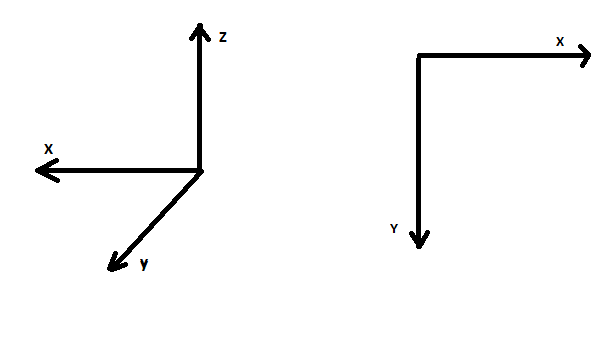
\includegraphics[width=0.6\textwidth]{figures/Vacuum/SistemaRef_world_image.png}
		\caption{Sistema de referencia del mundo (izquierda) y sistema de referencia de la imagen (derecha)}
		\label{fig.sistemaref_world}
		\end{center}
\end{figure}

Para poder saber dónde está situado nuestro robot en la imagen tenemos que pasar de una coordenada (x, y) en 3D a una coordenada (x’, y’) en 2D. Para poder pasar de un sistema en 3D a un sistema 2D se ha aplicado una matriz de rotación y traslación. En concreto, se aplica una rotación de pi grados (será el ángulo \(\alpha\) de la matriz) sobre el eje y. La traslación se realiza porque queremos tener el punto (0,0) de la imagen en la esquina superior izquierda, y para que se corresponda correctamente cada punto de la imagen con cada punto del mundo. En este caso la traslación que se ha aplicado es de 0.6 (será tx) en el eje x; y -1 (será ty) en el eje y. La matriz de rotación y traslación sobre el eje y es la siguiente:\\

\begin{equation}
\left[\begin{array}{cc}
x' \\ 
y' \\
z' \\
1
\end{array}\right] = \left[\begin{array}{cccc}
\cos(\alpha) & 0 & \sin(\alpha) & tx \\ 
0 & 1 & 0 & ty\\
-\sin(\alpha) & 0 & \cos(\alpha) & tz \\
0 & 0 & 0 & 1
\end{array}\right]* \left[\begin{array}{cc}
x \\ 
y \\
z \\
1
\end{array}\right]
\end{equation}
\\

De esta forma podemos pintar el triángulo que es la representación de la aspiradora en la casa, pasando la coordenada del mundo que nos devuelve el pose3d a coordenada en la imagen, la cual será el centro del triángulo que dibujaremos con una pequeña desviación. El triángulo es un triángulo isósceles para poder distinguir cuál es la orientación del robot. La aspiradora estará orientada hacia el vértice que posee un ángulo menor que el resto.\\

Esta rotación también nos sirve para poder pintar en azul los puntos del mapa por donde ha pasado la aspiradora en cualquier momento. Se pintará un círculo en cada iteración dado que la aspiradora ocupa un determinado volumen. Los puntos por los que ha pasado la aspiradora se guardan en un array para poder saber por dónde ha pasado y pintarlos todos en cada iteración.\\

Por otra parte, en la esquina superior derecha de la GUI, tenemos un teleoperador para teleoperar el robot. Este teleoperador controla las velocidades lineal y angular del robot. La velocidad lineal del robot se puede controlar moviendo el joystick en sentido vertical. Cuanto más subamos el joystick más velocidad tendrá el robot hacia delante, y si lo bajamos del todo más velocidad lineal tendrá el robot hacia atrás. La velocidad angular del robot se controla moviendo el joystick en sentido horizontal, según lo movamos a izquierda o a la derecha, el robot girará en un sentido u otro.\\

En la aplicación gráfica hay dos botones, que son bastante importantes para la práctica. El botón superior que aparece con un símbolo de stop es el botón que emplearemos cuando teledirigimos a la aspiradora y queremos que pare en un punto y no siga navegando. El botón inferior, en el cual pone ``Run my algorithm'', es el botón con el que le ordenaremos a la práctica que comience a ejecutar la solución que se ha programado en el fichero MyAlgorithm.py. Si queremos que este código pare un determinado momento, pulsaremos el mismo botón haciendo que pare; y si queremos reanudar su comportamiento lo volveremos a pulsar.\\

Podemos ver cómo es esta interfaz nada más ejecutar la práctica en la figura 5.5, y podemos ver cómo es transcurrido un tiempo en la figura 5.6.\\

\begin{figure}[H]
  \begin{center}
    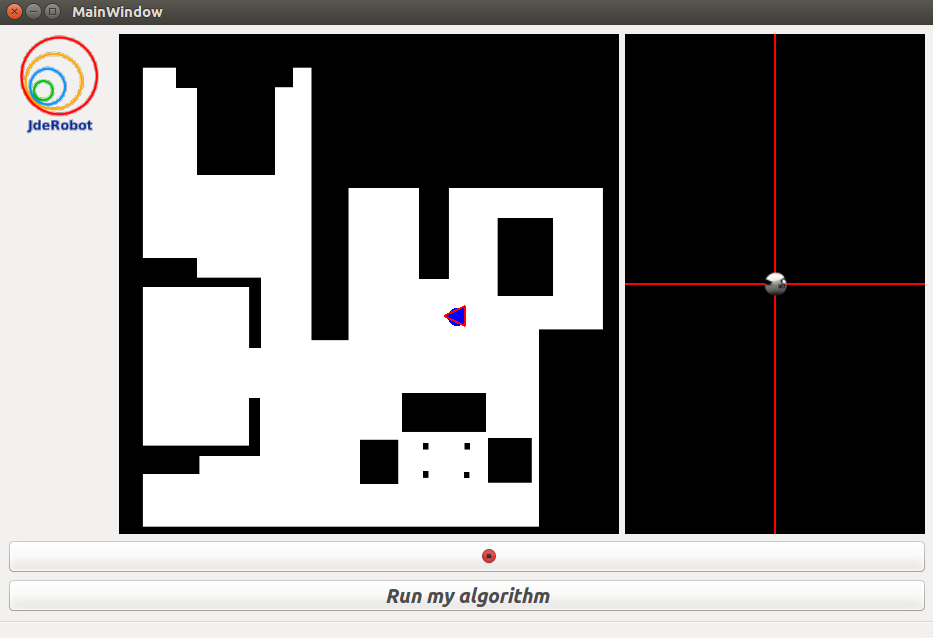
\includegraphics[width=0.7\textwidth]{figures/Vacuum/GUI_Vacuum.png}
		\caption{Interfaz gráfica (GUI) de Vacuum al iniciarse}
		\label{fig.GUI_Vacuum}
		\end{center}
\end{figure}

\begin{figure}[H]
  \begin{center}
    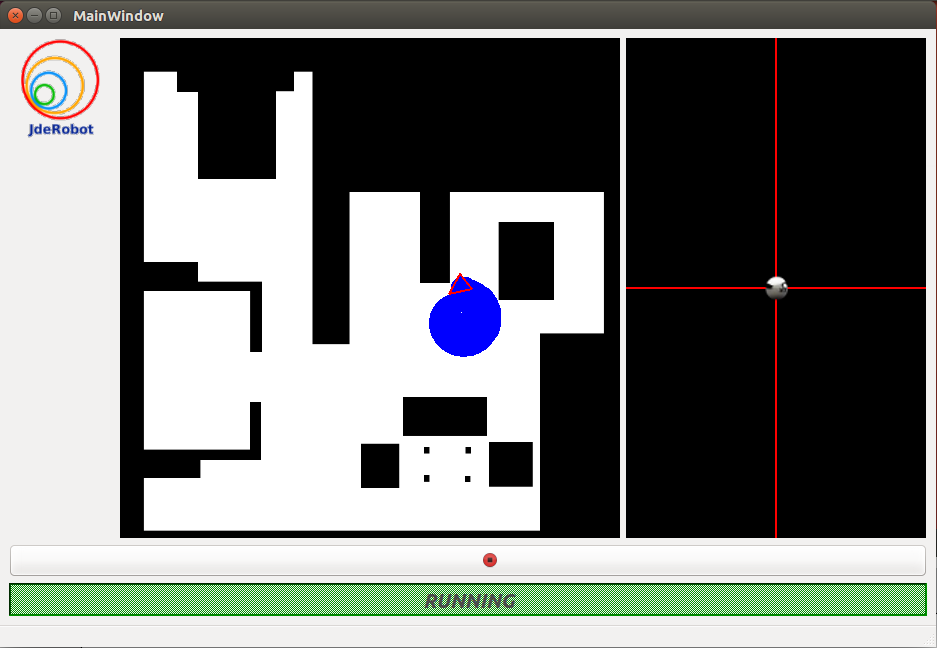
\includegraphics[width=0.7\textwidth]{figures/Vacuum/GUI2.png}
		\caption{Interfaz gráfica (GUI) de Vacuum después de un tiempo de ejecución}
		\label{fig.GUI2}
		\end{center}
\end{figure}

\section{Gráfica de la derivada del porcentaje}
En esta práctica se ha decidido crear una gráfica de la derivada del porcentaje en función del tiempo para poder comprobar cómo evoluciona el porcentaje de casa recorrido durante el tiempo.\\

La derivada de y (se representa en el eje vertical) respecto a x (se representa en el eje horizontal) es lo que varía y por cada unidad que varía x. Se puede designar este valor como dy/dx. Las expresiones dy y dx se llaman, respectivamente, diferencial de y, y diferencial de x. dx es la variable independiente y dy la variable dependiente de la función diferencial. Es decir, podemos ver que la derivada representa la diferencia de y respecto la diferencia de x. \\

En el caso de nuestra práctica, siguiendo esta definición de la derivada, podemos definir la derivada del porcentaje (eje vertical) respecto del tiempo (eje horizontal) como la diferencia del porcentaje cada unidad de diferencia del tiempo.\\

En la práctica en el eje vertical se representa la diferencia del porcentaje cada cierto tiempo. En el eje horizontal se representan las diferencias de tiempo, que siempre representan el mismo intervalo de tiempo. \\

En este caso, en el eje horizontal se representa el tiempo, el cual se divide en 9 intervalos de tiempo. Cada intervalo de tiempo que se representa, en el eje horizontal, se corresponde con un intervalo de 100 segundos. Por lo tanto, en la práctica vamos a observar el comportamiento del porcentaje a lo largo de 900 segundos, es decir, 15 minutos.\\

En el eje vertical, se representa la diferencia de porcentaje en cada intervalo de tiempo. Es decir, por ejemplo, en el primer intervalo de tiempo se representará la diferencia de porcentaje recorrido entre el segundo 100 de la práctica y el segundo 0. Así, sucederá para cada uno de los intervalos.\\

De esta forma, esta gráfica nos permitirá ver cómo evoluciona el porcentaje recorrido respecto al tiempo. Cuando la aspiradora realiza el algoritmo de navegación puede que en ciertas ocasiones pase varias veces por una misma zona o se quede un rato atascada en ciertas zonas. Es decir, que al principio cuando ejecutamos la práctica es muy sencillo que nuestra aspiradora recorra un gran porcentaje de casa, pero más adelante será más complicado que pase por zonas por las que no había pasado. Esto implica que posiblemente la derivada del porcentaje en función del tiempo sea mayor al comienzo de la ejecución de la práctica que por el final. Cada vez que se ejecute la práctica esta gráfica variará.\\

Esta gráfica tendrá 9 escalones en el eje horizontal como hemos mencionado antes, y 5 escalones (cada uno representa una diferencia del 2\%) en el eje vertical. La gráfica se representa en color rojo. En la imagen 5.7 podemos ver cómo se muestra la gráfica cuando acabamos de ejecutar la práctica. En la imagen 5.8 se puede observar un ejemplo de la gráfica de la derivada del porcentaje recorrido en función del tiempo.\\

\begin{figure}[H]
  \begin{center}
    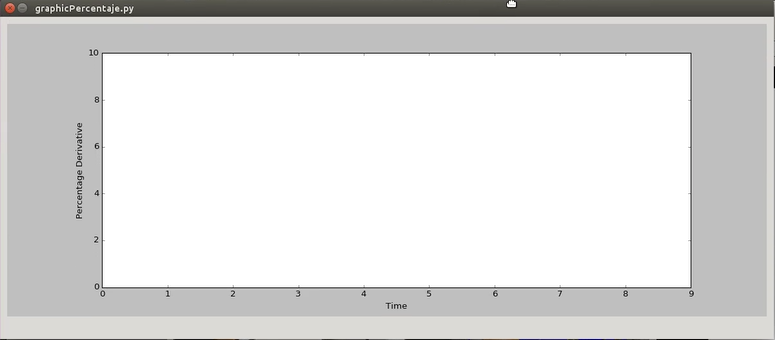
\includegraphics[width=0.9\textwidth]{figures/Vacuum/Grafica_percentaje1.png}
		\caption{Gráfica de la derivada del porcentaje en función del tiempo al ejecutar la práctica}
		\label{fig.grafica_percentaje1}
		\end{center}
\end{figure}

\begin{figure}[H]
  \begin{center}
    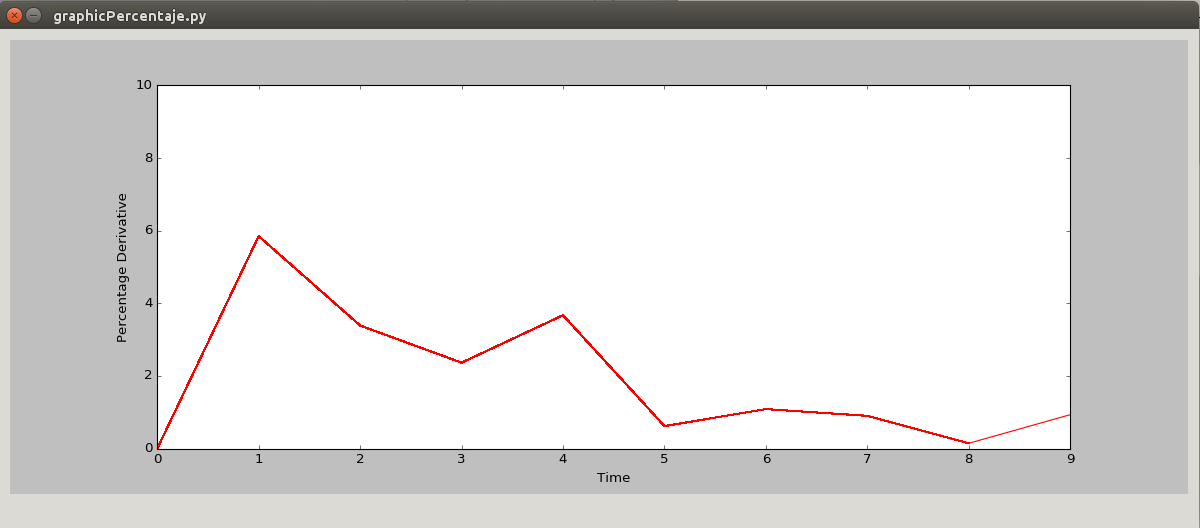
\includegraphics[width=0.9\textwidth]{figures/Vacuum/Grafica_percentaje2.png}
		\caption{Gráfica de la derivada del porcentaje en función del tiempo}
		\label{fig.grafica_percentaje2}
		\end{center}
\end{figure}

\section{Árbitro}
En esta práctica se ha creado un árbitro, que en función de diferentes parámetros califica el algoritmo que programa el alumno como solución. El árbitro muestra en una interfaz gráfica diferentes parámetros, así como la nota que obtiene el alumno. Este árbitro se ha creado utilizando PyQt5 al igual que la aplicación gráfica. Para programar el árbitro se han creado clases diferentes para cada parámetro que queramos mostrar en la interfaz. Estas clases serán instanciadas en una clase principal (llamada MainWindow), que será la clase que contiene la ventana principal de la aplicación del árbitro.\\

En la esquina superior izquierda, la aplicación del árbitro tiene un visor que muestra una barra de progreso. En esta barra se pinta en rojo el porcentaje de superficie recorrida por la aspiradora en cada momento. Encima de esta barra se mostrará un mensaje con el tanto por ciento de superficie recorrida. El porcentaje de superficie recorrida se calcula teniendo en cuenta que el 100\% de superficie que puede recorrer la aspiradora es el suelo donde no hay obstáculos situados. Es decir, el 100\% de superficie que se puede recorrer son todos los píxeles en blanco que aparecen en el mapa que muestra la interfaz.\\

En la esquina inferior izquierda de la aplicación se muestra la imagen del mapa de la casa. Esta imagen es una imagen binaria, en la cual los píxeles blancos (valor 255) representan la zona libre de obstáculos por donde puede navegar la aspiradora (el suelo). Los píxeles en negro (valor 0) representan a los obstáculos que hay en la casa. En esta imagen también se pinta en azul las zonas por donde ha pasado la aspiradora en cualquier momento. Para ello se guardan las posiciones por las que pasa en un array, y se pinta en cada iteración.\\

En la esquina superior derecha de la aplicación, tenemos un visor que muestra un reloj digital. En este reloj se muestran segundos, pero estos segundos no van aumentando según va pasando el tiempo. Por el contrario, los segundos van disminuyendo, es decir, se muestra una cuenta atrás de segundos. Este visor comienza mostrando 900 segundos (que son 15 minutos) y cada vez que ha pasado un segundo lo va descontando de este valor. Se muestran 15 minutos porque se ha considerado un intervalo de tiempo adecuado para evaluar la práctica, ya que si pusiéramos un intervalo mayor de tiempo sería un tiempo excesivo para evaluar la práctica. Sin embargo, si ponemos un intervalo de tiempo menor a 15 minutos no se podría evaluar la práctica con claridad, ya que en los primeros minutos de la práctica es muy sencillo recorrer bastante porcentaje de suelo comparando con los minutos posteriores.\\

Debajo de este visor del tiempo digital se muestra un visor de un reloj analógico. En este reloj analógico sí que avanza el tiempo, al contrario que sucedía con el reloj digital. Este tiene pintadas 60 “rayitas” que se corresponden con 60 segundos. En este reloj aparecen pintadas dos manecillas, la más alargada se corresponde con la manecilla de los segundos, y la más corta con la manecilla de los minutos. Conforme haya pasado un segundo la manecilla de los segundos apuntará al siguiente segundo. Lo mismo sucederá con la manecilla de los minutos.\\

En la esquina inferior derecha, se representa una imagen del logo de JdeRobot. Esta imagen es una imagen RGB y ha sido escalada a un tamaño menor.\\

Por último, hay que mencionar que cuando terminen los 900 segundos, a la derecha del reloj digital aparecerá un mensaje con la nota que ha obtenido el alumno. Esta nota se calculará en función del porcentaje recorrido por la aspiradora al pasar 900 segundos. Se ha establecido un porcentaje máximo para estos 15 minutos, ya que no es posible recorrer toda la casa en este tiempo. Este porcentaje es de 30\%. Si la aspiradora recorre un 30\% o más, el alumno obtendrá una nota de 10 puntos. Si por el contrario, la aspiradora recorre menos porcentaje, entonces se calcula la nota haciendo una regla de tres sabiendo que una nota de 10 es un 30\%.\\

En las imágenes 5.9, 5.10 y 5.11, podremos ver el árbitro al inicio de la práctica, el árbitro durante el pilotaje, y tras la evaluación de la práctica.\\

\begin{figure}[H]
  \begin{center}
    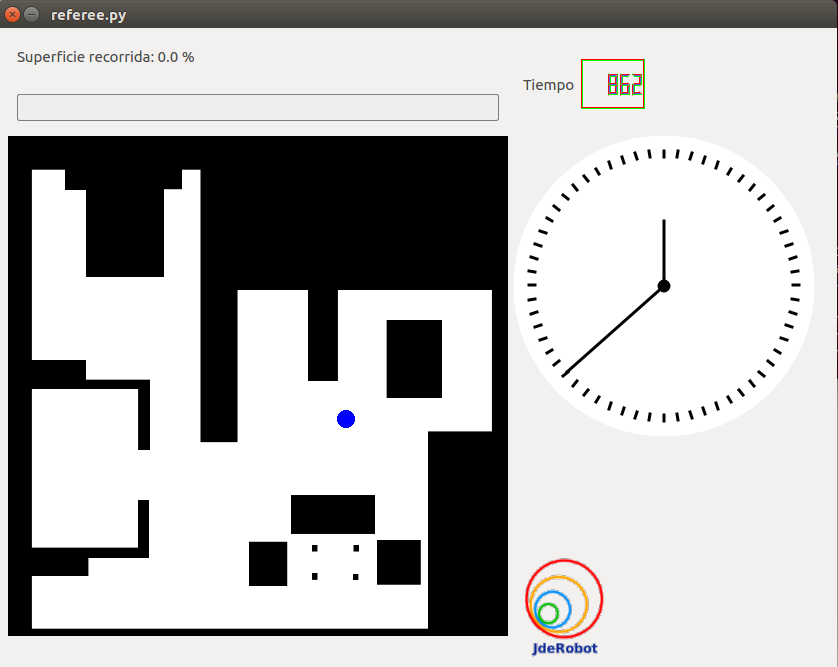
\includegraphics[width=0.6\textwidth]{figures/Vacuum/Referee_Vacuum.png}
		\caption{Árbitro al inicio de la práctica}
		\label{fig.Referee_Vacuum}
		\end{center}
\end{figure}

\begin{figure}[H]
  \begin{center}
    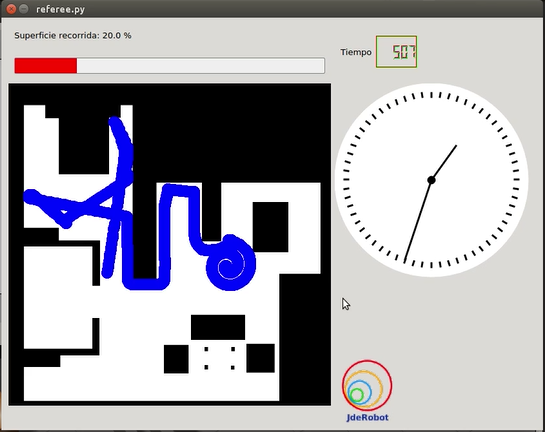
\includegraphics[width=0.6\textwidth]{figures/Vacuum/Referee_Vacuum2.png}
		\caption{Árbitro durante la ejecución de la práctica}
		\label{fig.Referee_Vacuum2}
		\end{center}
\end{figure}

\begin{figure}[H]
  \begin{center}
    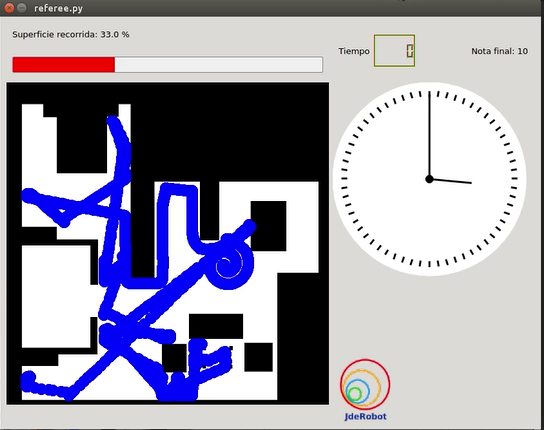
\includegraphics[width=0.6\textwidth]{figures/Vacuum/Referee_Vacuum_3.png}
		\caption{Árbitro tras evaluar la práctica}
		\label{fig.Referee_Vacuum3}
		\end{center}
\end{figure}

\section{Solución}
\subsection{Algoritmo empleado por distintas aspiradoras robóticas}
En los últimos 15 años, han aparecido múltiples modelos de aspiradoras robóticas, las cuales son cada vez más innovadoras. Es importante tener en cuenta los algoritmos de navegación que llevan a cabo cada uno de los modelos, ya que en función de estos algoritmos la aspiradora limpiará en menor o mayor tiempo la casa. Además, es importante tener en cuenta en estos algoritmos los posibles obstáculos con los que se encontrará la aspiradora al recorrer la casa. A continuación, podemos ver diferentes algoritmos de navegación que existen hoy en día en función del modelo:

\begin{itemize}
\item Uno de los primeros modelos de aspiradora Trilobite de Electrolux navega empleando ultrasonidos. Esta aspiradora usa la siguiente estrategia de navegación: explora el perímetro del entorno (siguiendo un comportamiento de sigue la pared); después de que la aspiradora llegue al punto de partida donde comenzó a recorrer la pared, el robot estima el tamaño del entorno y comienza con una trayectoria aleatoria.\\
\begin{figure}[H]
  \begin{center}
    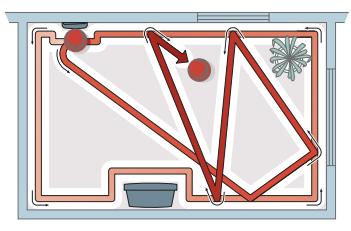
\includegraphics[width=0.6\textwidth]{figures/Vacuum/Trilobite.png}
		\caption{Patrón de navegación de la aspiradora Trilobite}
		\label{fig.Trilobite}
		\end{center}
\end{figure}
\item El sistema de navegación de la aspiradora robótica Xiaomi está guiado por un láser. Utiliza el algoritmo Simultaneous Localization and Mapping (SLAM) para generar un mapa de la casa en la que se encuentra y calcula patrones inteligentes para moverse a través de la casa. Xiaomi afirma que su modelo de aspiradora no solamente sigue un mapa y trata de limpiar el 100\% de la superficie del suelo de la casa, simplemente siguiendo las instrucciones, sino que en realidad su aspiradora puede pensar y calcular el mejor patrón de limpieza para la casa.  Cuando arranca Xiaomi, hace un escaneo de la zona circundante y divide la habitación en secciones de aproximadamente 4 por 4 metros. A continuación, el robot realiza un barrido del perímetro alrededor de esta área seccionada, trazando los obstáculos que puedan interponerse en el camino de la trayectoria. Después, ``rellena'' esta sección haciendo barridos horizontales.\\
\begin{figure}[H]
  \begin{center}
    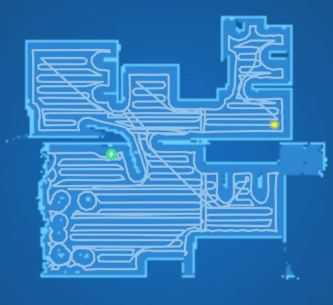
\includegraphics[width=0.4\textwidth]{figures/Vacuum/Xiaomi.png}
		\caption{Patrón de navegación de la aspiradora Xiaomi}
		\label{fig.Xiaomi}
		\end{center}
\end{figure}
\item También es importante destacar la gama de robot LG Hombot. Vamos a analizar en concreto el sistema de navegación del LG Hombot Turbo. Este aspirador es capaz de crear un mapa de la superficie, memorizando cada obstáculo, evitando el movimiento aleatorio y minimizando los choques.
\item El más conocido de las aspiradoras robóticas es Roomba de iRobot. Roomba posee diferentes modelos, desde los más antiguos hasta los más innovadores. Existen grandes diferencias entre estos en cuanto a su patrón de limpieza. Los modelos de las series 500, 600, 700 y 800, calculan la ruta de limpieza óptima y determinan cuándo es necesario utilizar sus diversos modos de limpieza: giro en espiral, seguimiento de paredes, cruce de habitación. En cambio, los modelos de la serie 900 de Roomba, tienen navegación iAdapt 2.0, se adaptan al entorno y disponen de localización visual para limpiar. A través de la localización visual, crea un mapa con referencias, para recorrer toda la casa y saber por dónde ha pasado y dónde tiene que ir. Limpia de forma eficiente en áreas abiertas moviéndose en líneas paralelas mientras que, gracias a los sensores, adapta su trayectoria cuando se necesita limpiando de forma eficiente.
\end{itemize}

Estos modelos que acabamos de mencionar son solamente unos pocos dentro de una amplia variedad de modelos de aspiradoras robóticas que existen hoy en día.\\

Es importante destacar que todos los modelos de aspiradora usan diferentes modos de limpieza (espiral, zig-zag, aleatorio, recorrer bordes, etc) en función de la zona de la casa donde se encuentren o en función de qué es lo que más le interesa a su dueño.\\

Con la descripción de los patrones que emplean las aspiradoras anteriores, podemos deducir que existen modelos de aspiradoras que emplean patrones aleatorios para poder limpiar la casa; y, por otro lado, hay otros modelos que inicialmente se construyen un mapa de la casa para recorrer la superficie de una forma más óptima.\\

\subsection{Algoritmo empleado por Roomba serie 500, 600, 700, 800}
Para resolver el algoritmo sin autolocalización que se plantea en la práctica nos hemos basado en el algoritmo de navegación que siguen los modelos de las series 500, 600, 700 y 800 de Roomba, que no emplean un mapa de la casa para poder realizar el algoritmo. A continuación, se explicará cómo navega Roomba por su entorno.\\

Mientras Roomba está limpiando evita caerse por las escaleras o por un terreno empinado. Esto lo hace gracias a cuatro sensores infrarrojos en la parte inferior delantera. Estos sensores envían constantemente señales de infrarrojos, y si estas señales se pierden es porque el robot ha llegado a una zona de elevada pendiente por donde podría caerse. De esta forma es como Roomba evita caerse por pendientes al dirigirse hacia otra zona.\\

Cuando Roomba choca con un objeto el bumper se retrae, activando sensores de objetos mecánicos que le avisan a Roomba de que ha chocado. Cuando se produce este hecho la aspiradora gira y avanza hasta que encuentra una ruta clara.\\

Esta aspiradora tiene otro sensor de infrarrojos (llamado Wall sensor) situado en la parte delantera del robot. Este sensor permite que Roomba navegue muy de cerca de las paredes, los objetos, etc. \\

Cuando presionamos el botón ``Clean'', lo primero que hace Roomba es calcular el tamaño de la habitación según la información que recibe a través de sus sensores. Este robot envía una señal infrarroja y comprueba el tiempo que tarda en volver la señal. De esta manera calcula el tiempo que tendrá que pasar limpiando. Esto le permite a Roomba optimizar la cobertura por habitación. El tiempo de funcionamiento depende del tamaño de la habitación y de la carga de la batería. Por lo que el robot sabe el tiempo que debe estar limpiando la habitación.\\

Roomba calcula su algoritmo 67 veces por segundo, obteniendo constantemente la información sobre su entorno y recomponiendo su trayectoria.\\

Roomba comienza a limpiar siguiendo un patrón de espiral. Esta espiral se va haciendo cada vez más grande, saliendo la espiral hacia fuera sobre un área más grande y más grande hasta que golpee un objeto. Cuando Roomba encuentre un objeto, seguirá a lo largo de este objeto recorriendo el perímetro de la habitación durante un periodo de tiempo determinado. Cuando pase este periodo de tiempo, Roomba comenzará el modo cruce de la habitación, tratando de averiguar la máxima distancia que puede navegar sin chocar con un objeto. Sin embargo, si lleva un periodo de tiempo grande navegando sin chocarse con ningún obstáculo va a comenzar otra vez a realizar la espiral, porque supone que está en un amplio espacio abierto.\\

Los patrones que eligieron los creadores de Roomba y como se desarrolló inicialmente se basan en los algoritmos basados en los comportamientos de los animales cuando van buscando áreas de comida.\\

Este algoritmo de navegación es bastante eficaz y robusto en situaciones del mundo real. A continuación, podemos observar en las imágenes el patrón de comportamiento que sigue la aspiradora Roomba.\\

\begin{figure}[H]
  \begin{center}
    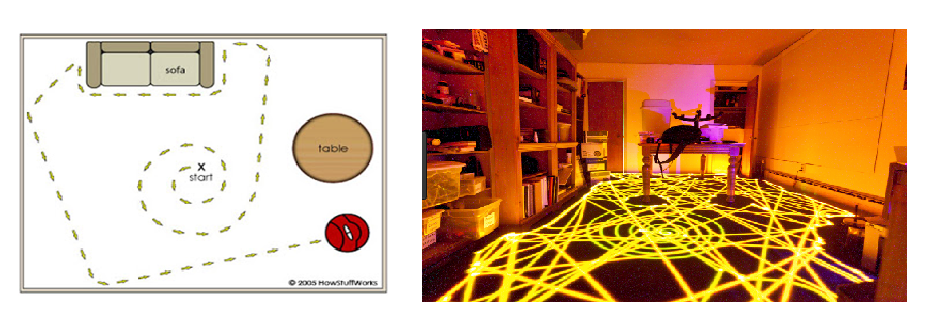
\includegraphics[width=1\textwidth]{figures/Vacuum/Algoritmo_roomba.png}
		\caption{Algoritmo de navegación de Roomba}
		\label{fig.Algoritmo_roomba}
		\end{center}
\end{figure}

\subsection{Solución desarrollada}
Las aspiradoras de hoy en día limpian de diversas formas, unas utilizan autolocalización, mientras que otras no. En el caso de esta práctica, el algoritmo de solución debe ser sin autolocalización, por lo que la aspiradora no conocerá el mapa de la casa, ni sabrá dónde está situada. Existen, también, muchos algoritmos donde las aspiradoras no tienen localización. Sin embargo, hemos optado por basarnos en el algoritmo que realizan los modelos 50, 600, 700 o 800 de Roomba de iRobot. La solución implementada se describirá a continuación. \\

La solución se desarrolla en el fichero ``MyAlgorithm.py''. En este fichero, la solución se desarrollará en el método ``execute'', el cual se ejecuta periódicamente. De esta forma, el pilotaje se llevará a cabo como un control reactivo, es decir, la aspiradora podrá comprobar los datos de sus sensores en cada instante y basándose en estos datos optar por realizar una acción u otra. En el caso de esta práctica, podemos ver que no se realiza ningún tipo de planificación, sino que se lleva a cabo el pilotaje directamente.\\

El primer paso que lleva a cabo Roomba, en la práctica, es realizar una navegación siguiendo un patrón en espiral (al igual que lo hacía la Roomba real). Si queremos realizar un patrón en espiral debemos elegir qué tipo de espiral queremos que intente realizar nuestra aspiradora, ya que existen numerosos tipos de espiral. Algunos de los tipos de espiral son: espiral de Arquímedes, espiral logarítmica, espiral hiperbólica, espiral de Fermat, espiral de Durero. En el caso de esta práctica se ha optado por realizar la espiral de Arquímedes, que es uniforme. Esta espiral se define como el lugar geométrico de un punto moviéndose a velocidad constante sobre una recta que gira sobre un punto de origen fijo a velocidad angular constante. En la imagen siguiente se puede ver el patrón que sigue la espiral de Arquímedes.\\

\begin{figure}[H]
  \begin{center}
    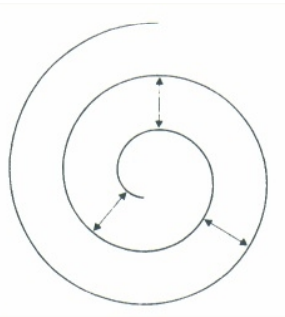
\includegraphics[width=0.3\textwidth]{figures/Vacuum/Espiral_Arquimedes.png}
		\caption{Espiral de Arquímedes}
		\label{fig.Espiral_Arquimedes}
		\end{center}
\end{figure}

Para que la aspiradora pueda realizar un patrón de este tipo, debe tener una velocidad angular constante y una velocidad lineal incremental. Es decir, la velocidad lineal irá aumentando en cada iteración un determinado valor. En el caso de esta práctica se ha optado por tomar como velocidad lineal la multiplicación de dos valores (los cuales inicialmente son valores muy pequeños). Un valor de radio inicial será multiplicado por una variable, la cual irá aumentando en cada iteración. El valor del radio inicial es de 0.1, mientras que la variable inicialmente posee un valor de 0.01. Esta variable será incrementada un 0.012 en cada iteración. De esta forma obtenemos un patrón en espiral similar a la espiral de Arquímedes.\\

Esta espiral se va haciendo cada vez más grande, saliendo la espiral hacia fuera sobre un área más grande. Roomba seguirá este patrón en espiral hasta que choque con un obstáculo. A continuación, podemos ver el patrón en espiral que ha realizado la aspiradora al ejecutar la práctica.\\

\begin{figure}[H]
  \begin{center}
    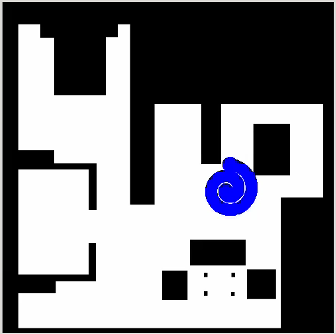
\includegraphics[width=0.5\textwidth]{figures/Vacuum/Espiral_Roomba.png}
		\caption{Espiral que realiza Roomba en la práctica}
		\label{fig.Espiral_Roomba}
		\end{center}
\end{figure}

Cuando Roomba choca con un obstáculo, sigue a lo largo de este obstáculo recorriendo el perímetro de la casa durante un determinado periodo de tiempo. En el caso de esta práctica, el periodo de tiempo que Roomba realiza el patrón del perímetro es de 300 segundos. Se ha optado por esta duración porque en las pruebas que se han realizado es el que mejores resultados presentaba.\\

Para poder seguir el perímetro se han empleado los datos que recoge el sensor láser que posee Roomba. Para poder obtener los datos del sensor láser se tiene que emplear la función laser.getLaserData(). Esta función nos devuelve 180 pares de valores, que se componen del ángulo y la distancia.\\

Lo primero que hace Roomba es separarse un poco de la pared para no rozar todo el rato con ella. Después gira un poco hasta que encuentra que tiene la pared a su derecha. Para saber si tiene la pared a la derecha emplea el valor de distancia del ángulo 0 (rayo del láser que está a la derecha de Roomba) y el ángulo 45 del array de 180 pares de valores, que mencionamos antes. Para obtener la distancia de cada ángulo se emplea la función distanceData[ángulo]. Un punto importante a tener en cuenta es que la distancia que devuelve el láser es en milímetros. \\

Tras saber que ya tenemos la pared a la derecha de la aspiradora, podemos recorrer el perímetro. Para ello hay que comprobar continuamente el láser frontal (situado en el ángulo 90). Este láser se comprueba para saber si la aspiradora está en una esquina, ya que en este caso la distancia que obtiene el láser será muy pequeña. Si se da el caso de que se encuentra en una esquina, Roomba girará a la izquierda 90 grados. \\

Otro dato que comprobará es si el láser del ángulo 135 (más a la izquierda) tiene una distancia muy pequeña y además ha detectado un choque. Esto supone que nuestra aspiradora se ha quedado enganchada en algún hueco. Si se da este caso la aspiradora retrocede un poco y gira hacia la izquierda 90 grados.\\

Si la aspiradora no se encuentra en una esquina y no se ha quedado atascada en algún hueco, entonces la aspiradora recorrerá el perímetro siguiendo la pared. Para ello, se comprueba el láser derecho (ángulo 0) y el láser del ángulo 45. Este algoritmo se realiza de forma reactiva comprobando continuamente los datos y tomando decisiones en base a ellos. Si la distancia a la pared es demasiado pequeña es que estamos muy pegados a la pared. En este caso la aspiradora gira un poco a la izquierda para no chocarse con la pared. Si el valor de distancia, por el contrario, es muy grande, entonces gira un poco a la derecha para no desviarse de la pared. Si la distancia a la pared no es ni muy pequeña, ni muy grande, es que podemos seguir adecuadamente la pared tomando una velocidad lineal constante y una velocidad angular nula.\\

Teniendo en cuenta todas estas situaciones que se pueden dar al recorrer la pared, la aspiradora recorre el perímetro correctamente. En la siguiente imagen se puede ver cómo después de realizar el patrón en espiral, Roomba ha realizado el perímetro durante un intervalo de tiempo.\\

\begin{figure}[H]
  \begin{center}
    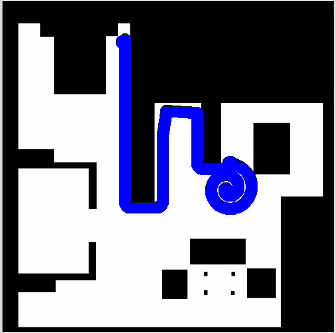
\includegraphics[width=0.5\textwidth]{figures/Vacuum/Perimetro_Roomba.png}
		\caption{Perímetro que recorre Roomba en la práctica}
		\label{fig.Perimetro_Roomba}
		\end{center}
\end{figure}

El siguiente paso que se lleva a cabo es un algoritmo aleatorio, que realiza un cruce de habitación (similar a la Roomba real). Lo que hace en este caso Roomba es comprobar si la aspiradora ha chocado o no continuamente, es decir, se comprueba si choca en cada iteración. Si ha chocado entonces la aspiradora retrocede un poco para apartarse de la pared, y calcula un ángulo aleatorio y el signo aleatoriamente. Este ángulo que se calcula aleatoriamente es el ángulo que girará Roomba para tomar una nueva orientación El signo que calculamos aleatoriamente es para que nuestra aspiradora gire algunas veces hacia la izquierda y otras veces a la derecha, dotando al algoritmo de mayor aleatoriedad. Para elegir el signo se emplea una función que proporciona Python para calcular aleatoriamente números enteros. En este caso se define un número entre 0 y 1. Si el signo sale 0, entonces Roomba gira a la derecha; si por el contrario es 1, gira a la izquierda.\\

Tras calcular el ángulo y el signo aleatoriamente, Roomba gira hasta haber girado el ángulo que se le ha indicado. Cuando ha realizado el giro, la aspiradora toma como velocidad de giro 0 y toma una velocidad lineal constante. De esta forma Roomba irá recta hacia la orientación que se haya quedado después del giro. Roomba seguirá la recta hasta que vuelva a chocar. Cuando choque volverá a realizar el algoritmo aleatorio hasta finalizar el tiempo de la práctica.\\

A continuación, se muestra la imagen del árbitro al finalizar el periodo de tiempo de la práctica. Se puede ver que se ha recorrido el 28 \% de la casa y que se ha obtenido en este caso una nota de 9.33. Tras esta imagen, tenemos otra imagen de la gráfica que representa la derivada en función del tiempo al finalizar la práctica.\\


\begin{figure}[H]
  \begin{center}
    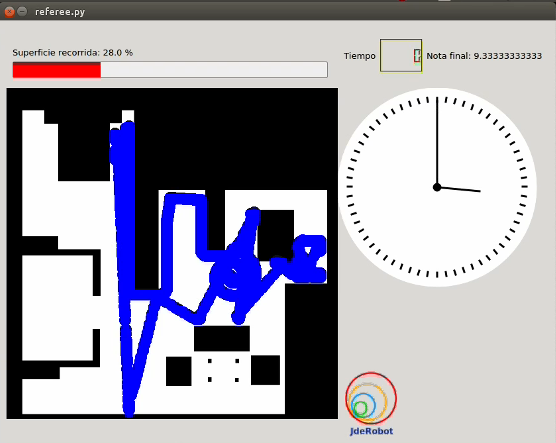
\includegraphics[width=0.6\textwidth]{figures/Vacuum/Referee_Roomba.png}
		\caption{Árbitro con la nota final}
		\label{fig.Referee_Roomba}
		\end{center}
\end{figure}

\begin{figure}[H]
  \begin{center}
    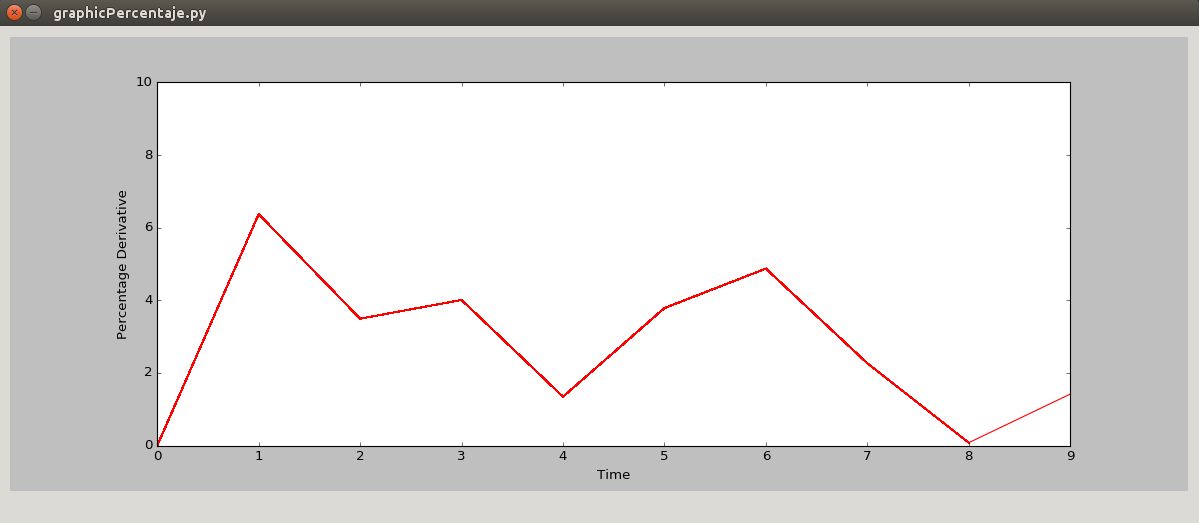
\includegraphics[width=0.9\textwidth]{figures/Vacuum/Porcentaje_Roomba.png}
		\caption{Gráfica de la derivada del porcentaje según en tiempo al finalizar la práctica}
		\label{fig.Porcentaje_Roomba}
		\end{center}
\end{figure}

En esta gráfica podemos ver cómo la derivada del porcentaje es mayor al comienzo de la práctica que en el resto de tiempo. Aunque se puede ver que hay algunos picos, donde baja su valor y luego aumenta.\\

\subsection{Experimentación}
En la práctica se decide evaluar 15 minutos, ya que un tiempo mayor supone demasiado tiempo para evaluar una práctica. Por el contrario, si fuera menor el tiempo, es muy probable que se obtuvieran resultados similares, ya que al comienzo de la práctica es más sencillo que aumente el porcentaje de suelo recorrido. Al ser un algoritmo en parte aleatorio, es probable que la aspiradora pase por un mismo sitio varias veces, por lo que no aumentará el porcentaje de superficie recorrida.\\

Un punto importante de la práctica es decidir cuál es el periodo de tiempo que la aspiradora recorrerá el perímetro. En la práctica se ha optado por recorrer el perímetro durante 300 segundos. Para poder elegir un periodo de tiempo se han hecho pruebas con diferentes periodos de tiempo en el que Roomba recorría el perímetro. Se han realizado tres pruebas por cada periodo de tiempo para sacar una media del porcentaje recorrido y elegir el periodo con mayor porcentaje, aunque al ser aleatorio si hiciéramos la prueba mil veces puede que saliera otro resultado, pero hemos elegido este periodo de 300 segundos en base a estas pruebas. Los periodos de tiempo en los que se han realizado pruebas para el perímetro son 200, 300, 400, 500 y 600 segundos.\\

En el caso del periodo de 200 segundos, se obtuvieron unos resultados del 20\%, 33\% y 18\%; lo que representa una media de un 23.66\% de la superficie de la casa. Si comprobamos las notas que se obtienen son de un 6.66, 10 y 6; obteniendo una nota media de 7.55. En este caso se puede ver que el 33\% es un gran resultado, que nos da como nota de calificación 10. Sin embargo, el resto de resultados obtenidos no son muy buenos, lo que hace que baje notablemente la nota. En la imagen 5.19 se puede ver la imagen del mapa con la superficie recorrida en azul para los 3 casos mencionados. En el caso de la segunda imagen se puede ver que hay más superficie recorrida.\\


\begin{figure}[H]
  \begin{center}
    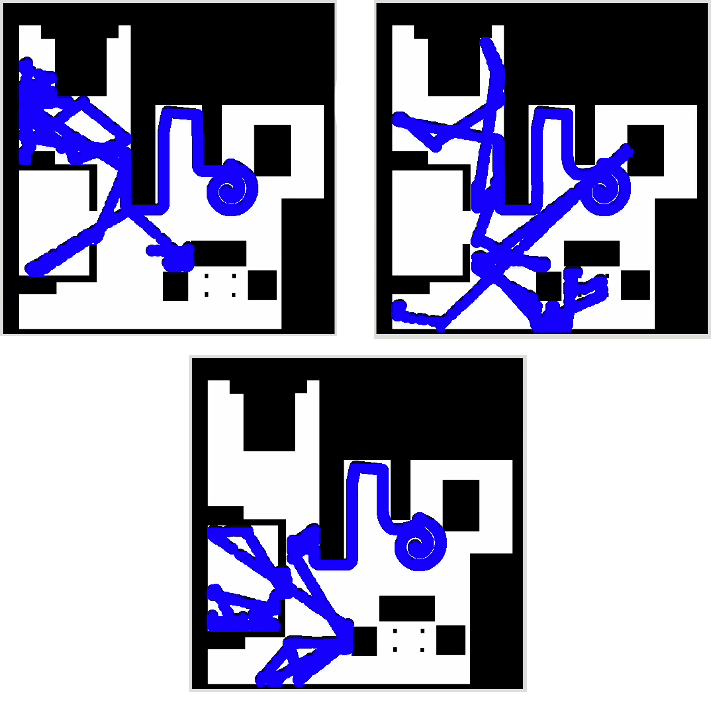
\includegraphics[width=0.7\textwidth]{figures/Vacuum/Referee200.png}
		\caption{Superficie recorrida de las pruebas de 200 segundos de perímetro}
		\label{fig.Referee200}
		\end{center}
\end{figure}

En la prueba del periodo de 300 segundos, se obtuvieron unos resultados de porcentaje de 28\%, 24\% y 27\%, lo que supone una media de porcentaje del 26.33\%. Las notas que se obtuvieron en estos casos son de 9.33, 8 y 9, dando como nota media un 8.77. Vemos que tanto la nota como el porcentaje, es mayor en este caso que en el periodo de 200 segundos. En este caso no hemos obtenido en ninguna prueba una nota de 10 como en el periodo de 200 segundos, pero la media es mejor. En la imagen 5.20 vemos el mapa con la superficie recorrida para las tres pruebas realizadas.\\

\begin{figure}[H]
  \begin{center}
    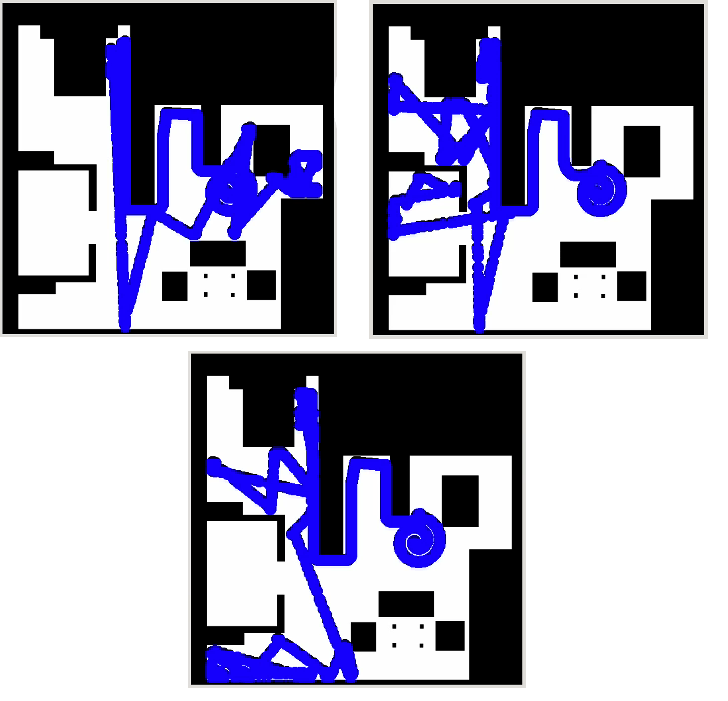
\includegraphics[width=0.7\textwidth]{figures/Vacuum/Referee300.png}
		\caption{Superficie recorrida de las pruebas de 300 segundos de perímetro}
		\label{fig.Referee300}
		\end{center}
\end{figure}

Cuando se han realizado pruebas con un periodo de 400 segundos para recorrer el perímetro, se han logrado porcentajes del 28\%, 14\% y 26\%, dando como media un porcentaje de 26\%. Las notas que se han obtenido como resultado han sido 9.33, 8 y 8.66, obteniendo como nota media un 8.66. Se puede observar que los resultados obtenidos en este caso son muy similares al periodo de 300 segundos, por lo que un periodo de 400 segundos también podría haberse empleado en la práctica, ya que da buenos resultados. En la imagen 5.21 se muestra el mapa con la superficie recorrida para cada una de las pruebas.\\

\begin{figure}[H]
  \begin{center}
    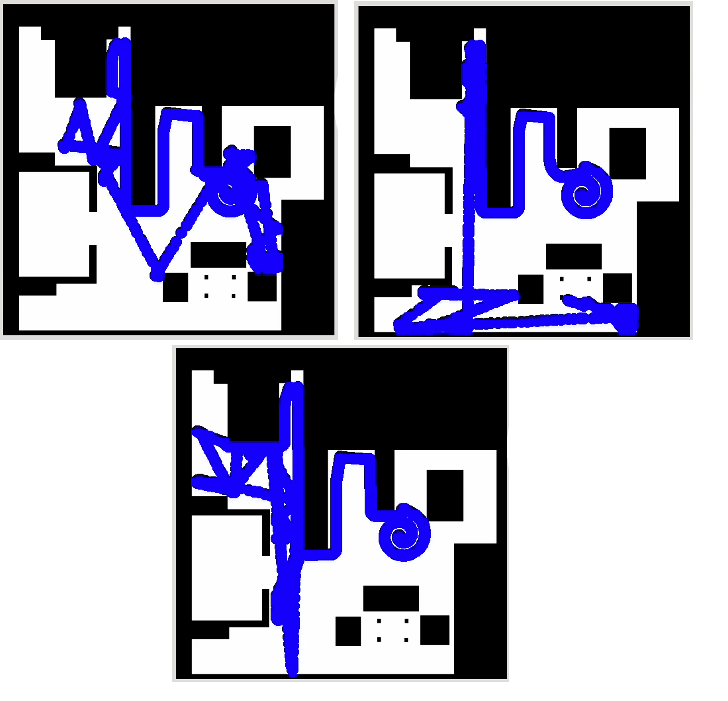
\includegraphics[width=0.7\textwidth]{figures/Vacuum/Referee400.png}
		\caption{Superficie recorrida de las pruebas de 400 segundos de perímetro}
		\label{fig.Referee400}
		\end{center}
\end{figure}

En el caso de emplear un periodo de 500 segundos, los porcentajes que se consiguen son del 20\%, 25\% y 18\%, lo que nos da una media de 21.66\%. Las notas que se logran con este periodo son 6.66, 8.33 y 6, dando como media un 7. Se puede ver que en el caso de este periodo de tiempo los resultados que se obtienen no son tan buenos como en los casos anteriores, por lo que se descartó usar este intervalo de tiempo. En la imagen 5.22 se ve el mapa con la superficie recorrida en cada caso.\\

\begin{figure}[H]
  \begin{center}
    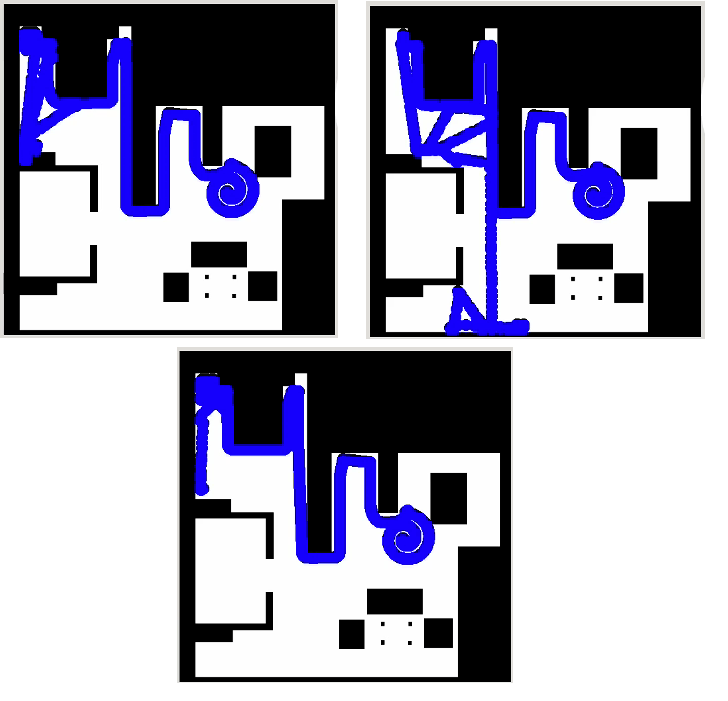
\includegraphics[width=0.7\textwidth]{figures/Vacuum/Referee500.png}
		\caption{Superficie recorrida de las pruebas de 500 segundos de perímetro}
		\label{fig.Referee500}
		\end{center}
\end{figure}

Por último, empleando un intervalo de tiempo de 600 segundos para recorrer el perímetro, logramos unos porcentajes de 22\%, 21\% y 22\%, dando como media un porcentaje de 21.66\%. En estas pruebas, las notas que se obtienen son de 7.33, 7 y 7.33; por lo que obtenemos una nota media de 7.22. Los resultados que se consiguen con este periodo de tiempo son similares a los obtenidos con un intervalo de 500 segundos. Podemos ver en la imagen 5.23 el mapa con la superficie recorrida por la aspiradora para las pruebas de 600 segundos. \\

\begin{figure}[H]
  \begin{center}
    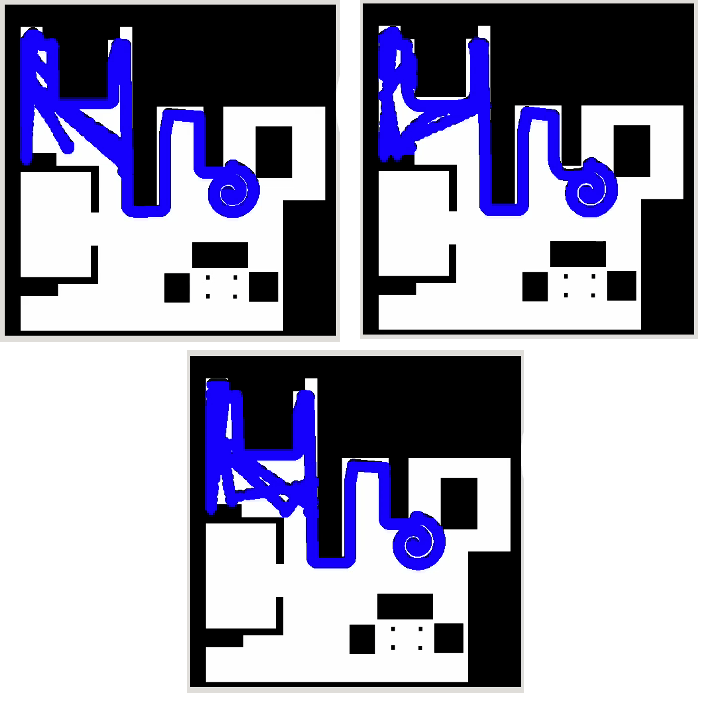
\includegraphics[width=0.7\textwidth]{figures/Vacuum/Referee600.png}
		\caption{Superficie recorrida de las pruebas de 600 segundos de perímetro}
		\label{fig.Referee600}
		\end{center}
\end{figure}

Es importante mencionar que, si tuviéramos una casa sin obstáculos, sin paredes y sin ningún hueco donde se pudiera quedar atascada la aspiradora, entonces el porcentaje que podría recorrer la aspiradora sería mucho mayor. Esto se debe a que estos inconvenientes hacen que la aspiradora se quede mucho tiempo en algunas zonas y no recorra otras. Es posible que la aspiradora navegue por una zona varias veces, y, sin embargo, no recorra otras zonas en estos 15 minutos.\\

Para comprobar la diferencia de porcentaje recorrido, se han hecho tres pruebas de 45 minutos, con el intervalo de perímetro de 300 segundos, por lo que la aspiradora realizará un algoritmo aleatorio durante mucho tiempo. \\

En las pruebas que se han realizado se han obtenido unos resultados de porcentaje del 49\%, 42\%, y 45\%. Estos porcentajes dan una media de 45.33\%. Por lo tanto, se puede ver que la media está cercana a la mitad de porcentaje de la casa. Por lo que se podría decir que si la aspiradora navegara durante hora y media podría llegar al 90\% o 100\% dependiendo de la ocasión. Aunque viendo que cada vez es más complicado alcanzar nuevos puntos en la casa por donde no haya pasado la aspiradora, probablemente tardará algo más. En la imagen 5.24 se puede ver el mapa con la superficie recorrida en las tres pruebas. En estas imágenes se puede observar que en algunas ocasiones hay algunas habitaciones donde la superficie ha sido recorrida casi en su totalidad.\\

\begin{figure}[H]
  \begin{center}
    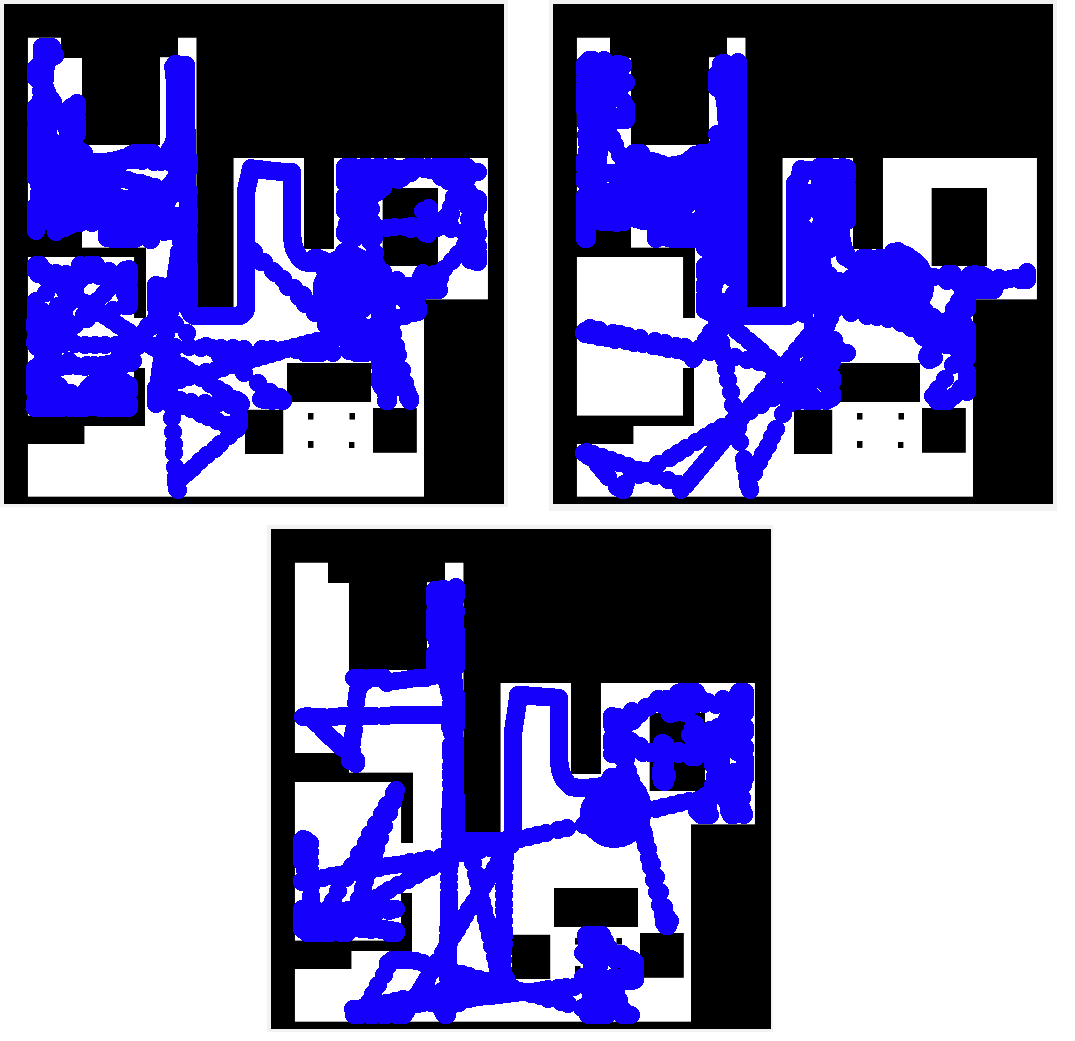
\includegraphics[width=0.7\textwidth]{figures/Vacuum/Referee_45MIN.png}
		\caption{Superficie recorrida de las pruebas de 45 minutos}
		\label{fig.Referee_45MIN}
		\end{center}
\end{figure}